\documentclass[12pt]{article}
%\usepackage[utf8]{inputenc}
%\documentclass[UTF8]{ctexart}
%\usepackage[UTF8, heading = false, scheme = plain]{ctex}
\usepackage{geometry}
%geometry{a4paper,scale=0.9}
\geometry{a4paper,left=1cm,right=1cm,top=1cm,bottom=2cm}
\usepackage{amsfonts}
\usepackage{color}
\usepackage{url}
%\usepackage{biblatex}
\usepackage{amsmath}
\usepackage{amssymb}
\usepackage{latexsym}
\usepackage[linesnumbered,ruled,lined]{algorithm2e}
\usepackage{cite}
%\addbibresource{ref.bib}
%\bibliography{ref.bib}
\usepackage{caption}
\usepackage{graphicx, subfig}
\usepackage{float}
%\usepackage[fontset=ubuntu]{ctex}
%\usepackage{fontspec}
\usepackage{xeCJK}
%\usepackage[colorlinks,
%anchorcolor=black,
%citecolor=black]{hyperref}
%\setmainfont{SimSun}
\usepackage[section]{placeins}
\usepackage{enumitem}
\usepackage{framed}
\usepackage[framemethod=TikZ]{mdframed}
\usepackage{indentfirst}
\usepackage{setspace}%使用间距宏包
\linespread{1.5}

\title{深入理解 Wide\&Deep 模型\cite{Understand_Wide_And_Deep_Model}}
\author{leolinuxer}
%\date{June 2020}

\begin{document}
%\setlength{\parindent}{0pt}
\maketitle
\tableofcontents

\section{Wide\&Deep模型简介}
\subsection{模型结构}
Wide\&Deep 由浅层(或单层)的Wide部分神经网络和深层的Deep部分多层神经网络组成,输出层采用softmax或logistics regression综合Wide和Deep部分的输出。
\begin{figure}[H]
    \centering
    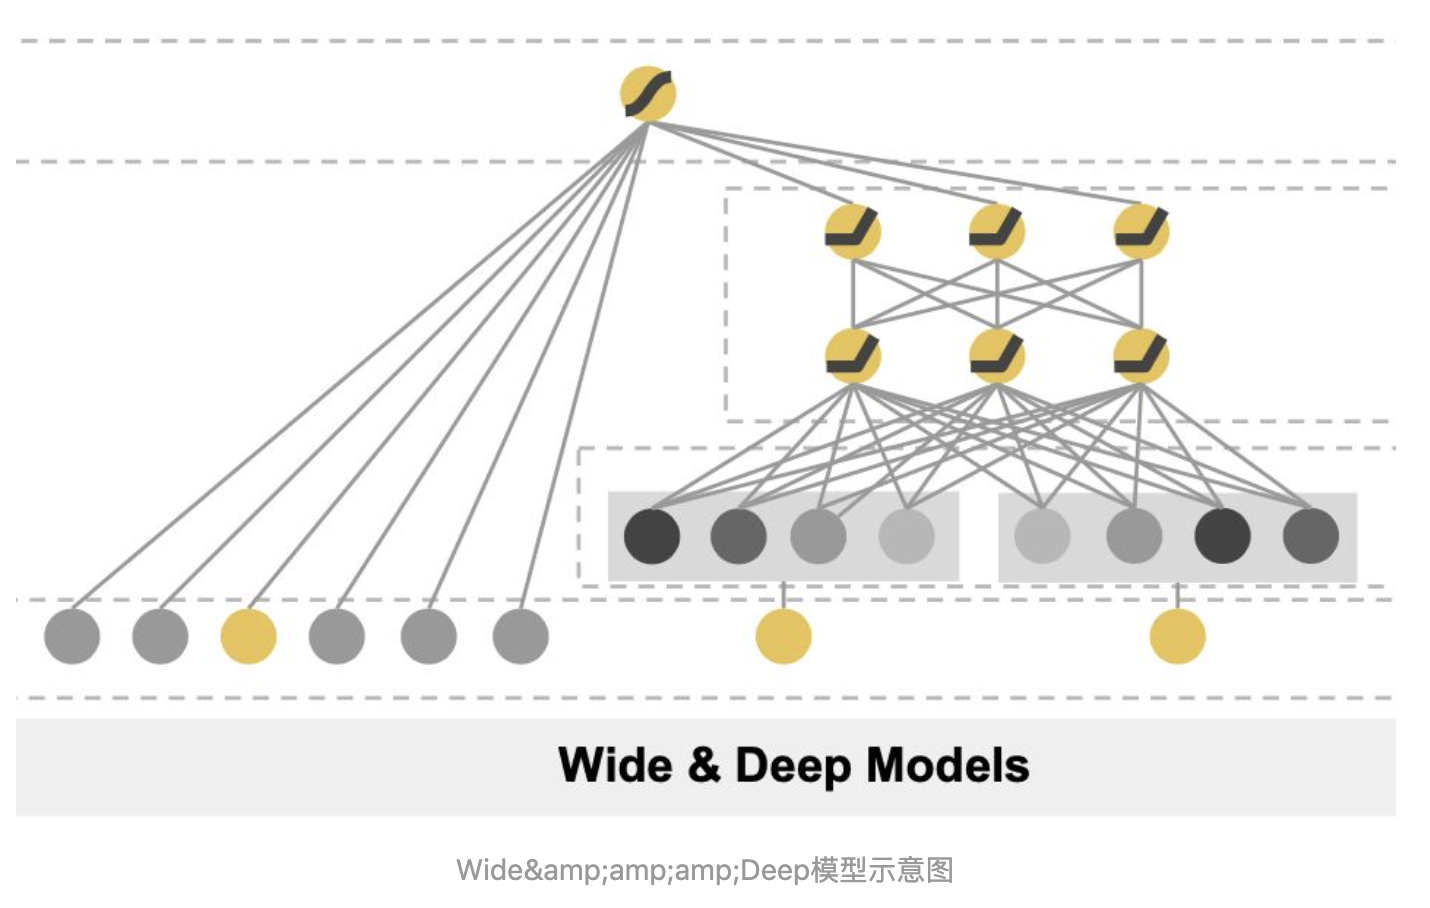
\includegraphics[width=1\textwidth]{fig/Wide_Deep_Structure.png}
\end{figure}

\subsection{模型特点}
\textbf{Wide部分有利于增强模型的“记忆能力”,Deep部分有利于增强模型的“泛化能力”。}

\section{为什么Wide\&Deep采用了不同的训练方法}

\begin{framed}
\textbf{为什么在Google的Wide\&Deep模型中,要使用带L1正则化项的FTRL作为wide部分的优化方法,而使用AdaGrad作为deep部分的优化方法?}

论文原文的描述是这样的:

In the experiments, we used Follow- the-regularized-leader (FTRL) algorithm with L1 regularization as the optimizer for the wide part of the model, and AdaGrad for the deep part.
\end{framed}

\subsection{为什么Wide部分要用L1 FTRL训练}
这里简要介绍一下,可以把 FTRL 当作一个\textbf{稀疏性很好,精度又不错的随机梯度下降方法}。由于是随机梯度下降,当然可以做到来一个样本就训练一次,进而实现模型的在线更新。所以在四五年前,大部分公司还是线性模型为主的时代,FTRL凭借非常好的在线学习能力成为主流。

说完了FTRL,再说L1正则化,参加过算法岗面试的同学可能都碰到过那个经典面试题“为什么L1正则化比L2正则化更容易产生稀疏解?”。问题的答案现在当然已经是显学了,但这里“稀疏”这个性质又冒出来了。也就是说FTRL with L1非常注重模型的稀疏性。这也就是问题的答案,W\&D采用L1 FTRL是想让Wide部分变得更加稀疏。

再白话一点就是,L1 FTRL会让Wide部分的大部分权重都为0,我们准备特征的时候就不用准备那么多0权重的特征了,这大大压缩了模型权重,也压缩了特征向量的维度。

\subsection{Wide部分的稀疏性为什么这么关键}
稀疏性不见得一直是一个好东西,它不管怎样都会让模型的精度有一定的损伤。肯定是特征向量维度过高导致“稀疏性”成为了关键的考量。这就涉及到Google Wide部分的特征选取了,到底Google选了什么特征需要这么注重稀疏性。我们回到他的业务场景中来。
\begin{figure}[H]
    \centering
    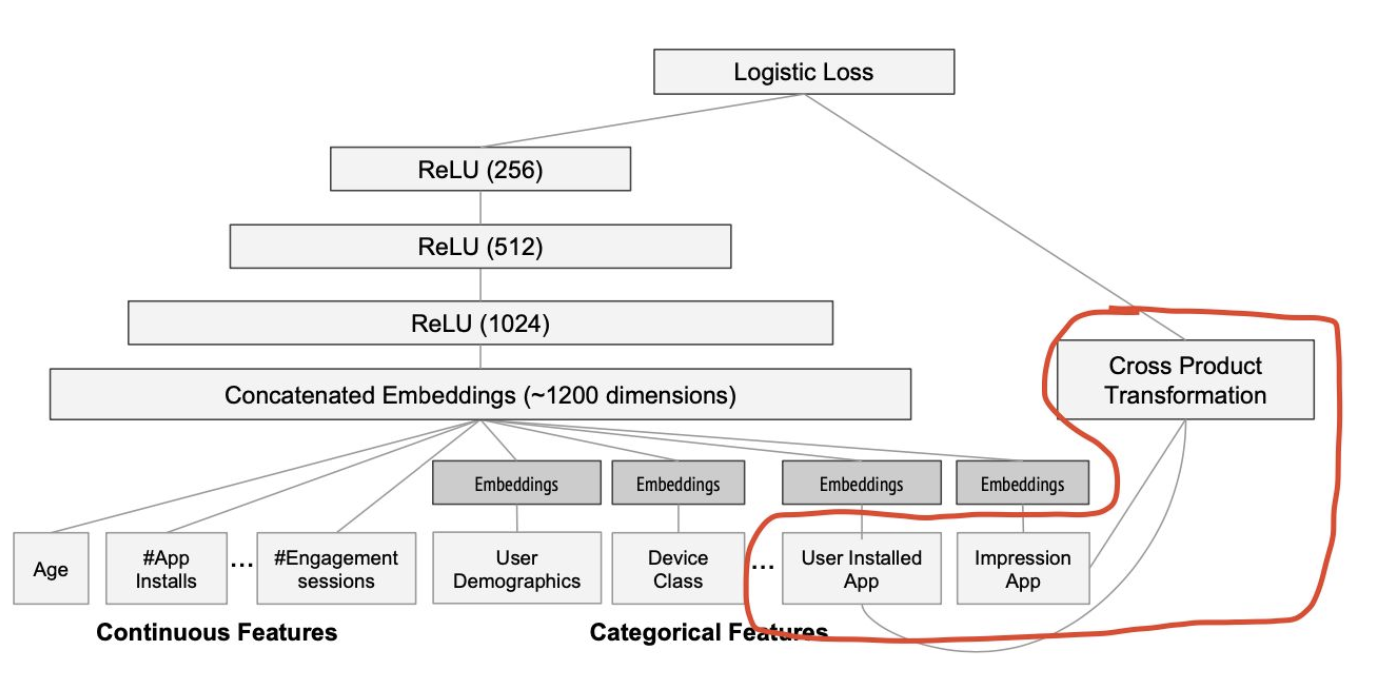
\includegraphics[width=1\textwidth]{fig/Wide_Deep_Structure_Detail.png}
\end{figure}

大家可以看到红圈内的Wide部分采用了两个id类特征的乘积,这两个id类特征是:
\begin{itemize}
\setlength{\itemsep}{0pt}
\setlength{\parsep}{0pt}
\setlength{\parskip}{0pt}
    \item User Installed App;
    \item Impression App;
\end{itemize}

这篇文章是Google的应用商店团队Google Play发表的,我们不难猜测Google的工程师使用这个组合特征的意图,他们是想发现当前曝光app和用户安装app的关联关系,以此来直接影响最终的得分。

但是两个id类特征向量进行组合,在维度爆炸的同时,会让原本已经非常稀疏的multihot特征向量,变得更加稀疏。正因如此,wide部分的权重数量其实是海量的。为了不把数量如此之巨的权重都搬到线上进行model serving,采用FTRL过滤掉哪些稀疏特征无疑是非常好的工程经验。

\subsection{为什么Deep部分不特别考虑稀疏性的问题}
大家注意观察可以发现Deep部分的输入,要么是Age,\#App Installs这些数值类特征,要么是已经降维并稠密化的Embedding向量,工程师们不会也不敢把过度稀疏的特征向量直接输入到Deep网络中。所以Deep部分不存在严重的特征稀疏问题,自然可以使用精度更好,更适用于深度学习训练的AdaGrad去训练。

\subsection{再说回模型的泛化能力和记忆能力}
再说回所谓wide部分的“记忆能力”。其实大家可以看到,所谓的“记忆能力”,可以简单理解为发现“直接的”、“暴力的”、“显然的”关联规则的能力。比如该问题中,Google W\&D期望在wide部分发现这样的规则:

用户安装了应用A,此时曝光应用B,用户安装的B概率大。

而Deep部分就更黑盒一些,它把能想到的所有特征扔进这个黑盒去做函数的拟合,显然这样的过程会“模糊”一些直接的因果关系,泛化成一些间接的,可能的相关性。

从这个角度来说,所谓“泛化能力”和“记忆能力”就更容易被直观的理解了。

\section{一些思考}
1. 如果lr时代特征工程做的很好,迁移到 deep,加 wide 部分收益不会太大,w\&d 可能更多的是给出一个简单通用的 lr 到 deep 的迁移框架。

2. 在实际应用时,可以考虑将 wide 和 deep 分开,在 deep 部分做 batch update 保证准确性和充足表达能力,wide 部分做 online learning 保证实效性;特别是对时效性要求高的时间段或场景,deep的效率跟不上,可以固定住deep,对wide进行online learning来增强记忆性

3. 如果直接把 deep 部分的 embedding 输入到 wide 侧可行吗;那就相当于 embedding 层后的 mlp 换成一层 lr 了,本质就是 deep 侧的 dnn。

%\printbibliography
\bibliography{../ref}
\bibliographystyle{IEEEtran}
\end{document}